鼠尾草属的名字Salvia源自于拉丁语词汇salvare,意为治疗师。该属包含多种具有药物活性的植物,自古以来就在世界上广泛用于治疗感冒、流感和月经失调。在土耳其民间医学中,鼠尾草属物种有驱风、利尿、止血、止痉、健胃的药效,并且因其抗菌和促进伤口愈合上的活性,亦被用于治疗口腔和咽喉炎症。世界上分布有超过900种鼠尾草属植物,其中58种为土耳其所特有。

土耳其女科学家Ulubelen和Topçu与她们的合作者研究了土耳其安纳托利亚(译注:亦称作小亚细亚)地区生长的鼠尾草属植物,并从中分离和表征出超过320种天然产物,其中大多数为萜类化合物,1/3为新报道的二萜类化合物。

\begin{figure}[h]
	\centering
	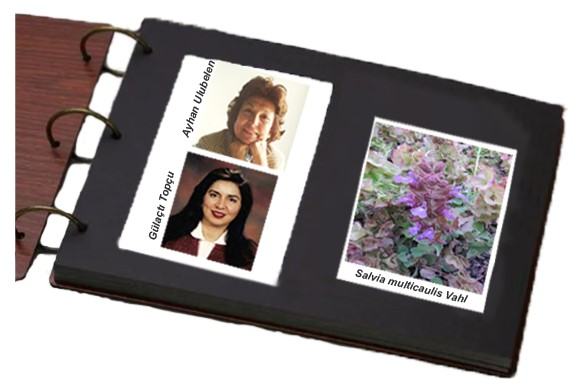
\includegraphics[width=12cm]{./pic/t1-1.jpg}
\end{figure}

在一篇关于\emph{Salvia multicaulis} Vahl.的研究中,Ulubelen和Topçu分离出了4种具有抗结核活性的全新芳香松香烷型二萜\textbf{1}--\textbf{4}。不仅分离出的二萜化合物具有抗细菌和抗真菌活性,植物提取物也显示出抗氧化、消炎和抑制胆碱酯酶的活性。\emph{S. multicaulis}在小亚细亚民间亦有使用,如作为开胃菜、用于促进伤口愈合,以及治疗蝎子叮咬、呼吸道感染、尿路感染和糖尿病等。

\begin{figure}[h]
	\centering
	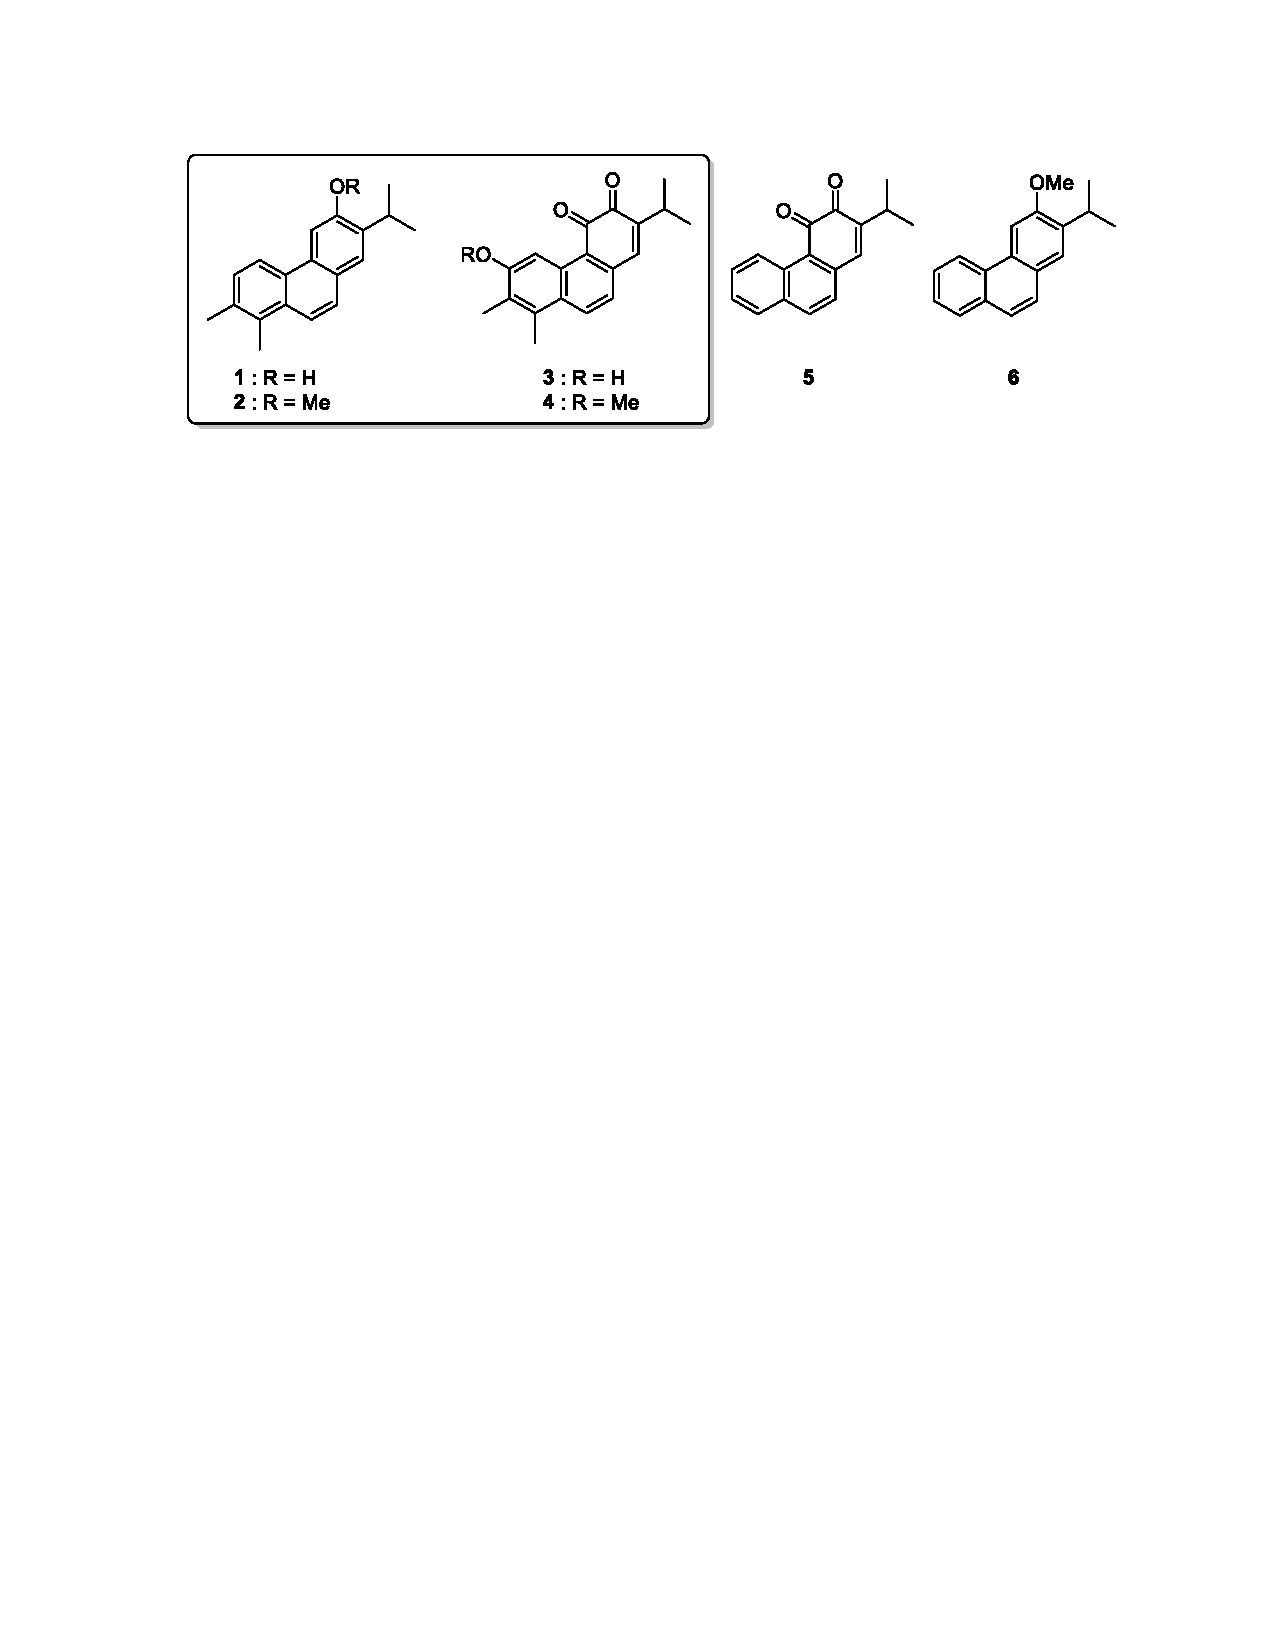
\includegraphics[width=14cm]{./pic/t1-2.pdf}
\end{figure}

随后一个土耳其的研究组发展了天然产物\textbf{1}--\textbf{4}衍生物的合成路线,本题就来源于此。合成二萜\textbf{1}和\textbf{5}的反应图如下所示。

\begin{figure}[h]
	\centering
	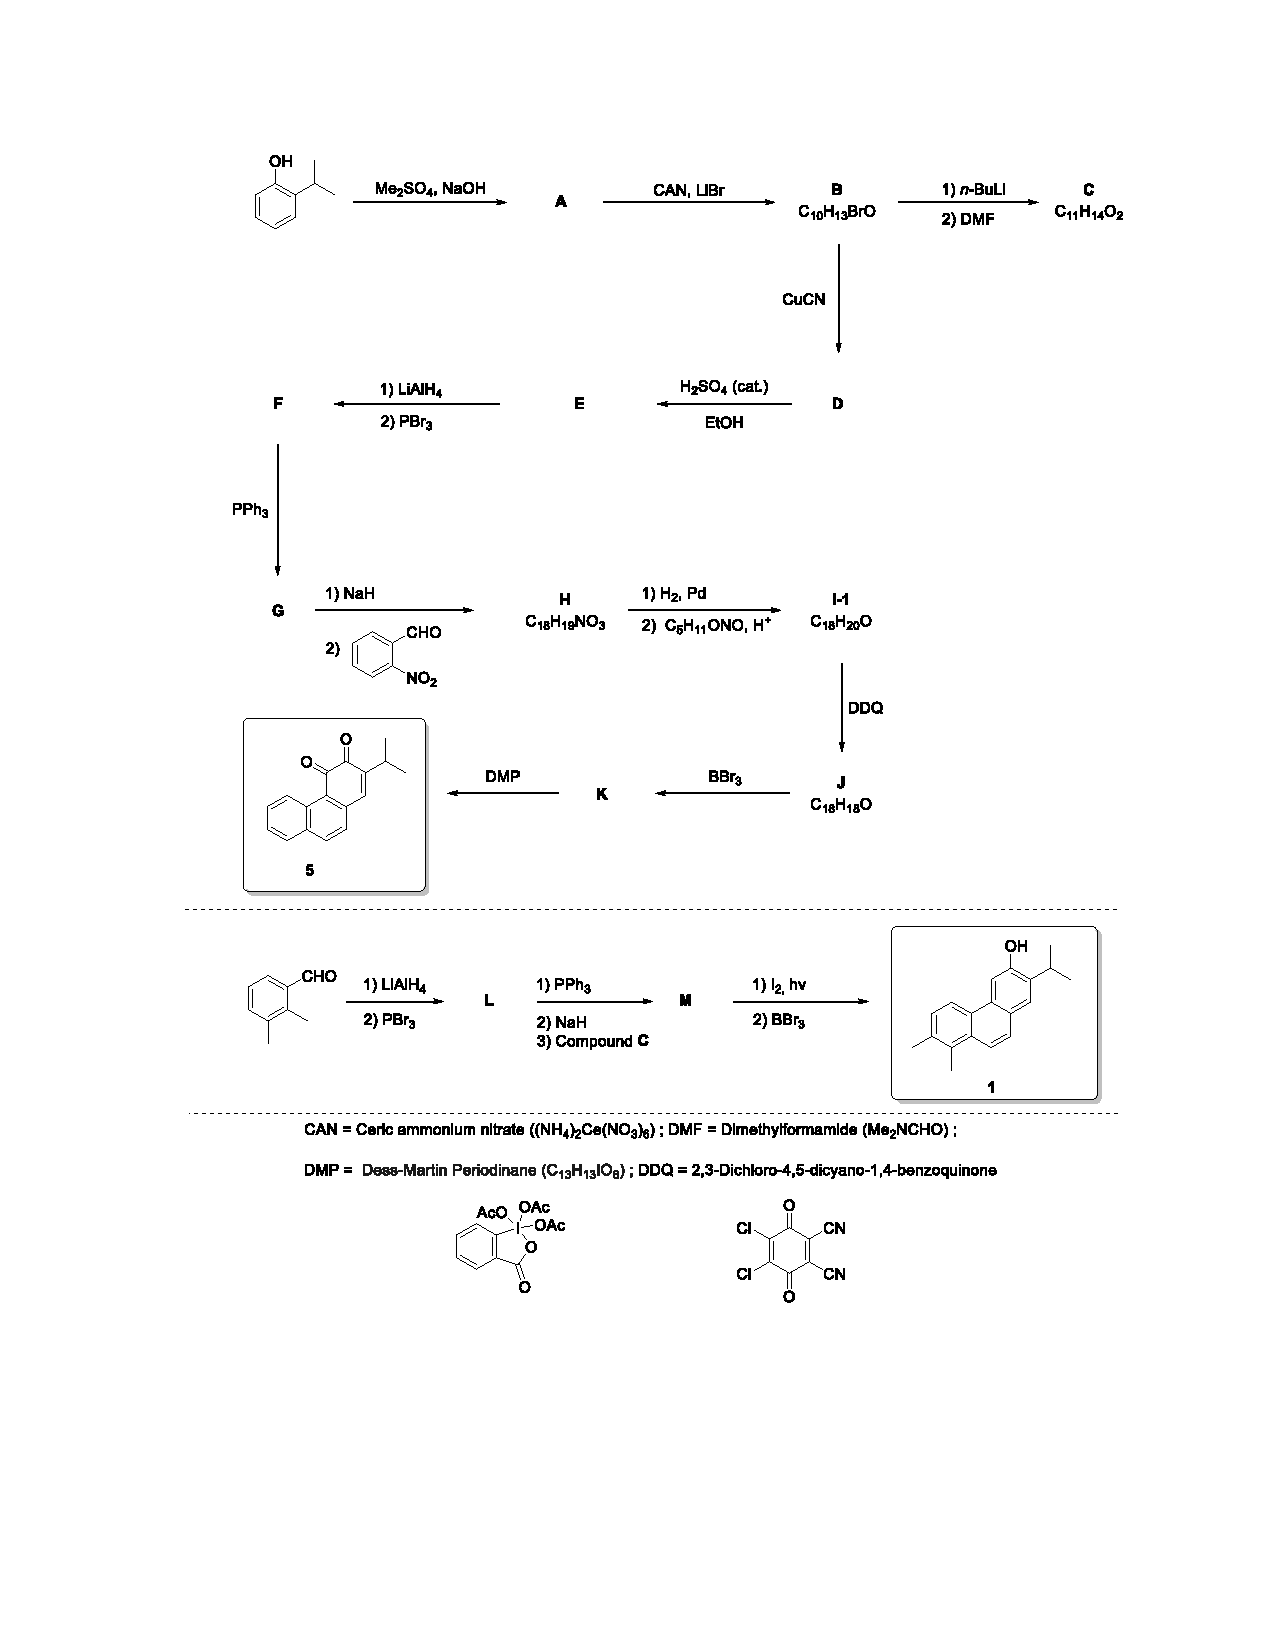
\includegraphics[width=16cm]{./pic/t1-3.pdf}
\end{figure}

\noindent\textbf{1.1.} 画出产物\textbf{A}--\textbf{M}的结构,无需考虑立体构型。\textbf{提示}:第二步 (\textbf{A}$\rightarrow$\textbf{B})中,溴化锂和硫酸铈(IV)铵合用作溴化试剂。化合物\textbf{C}是苯甲醛衍生物并用于化合物\textbf{M}的多步合成中。

\noindent\textbf{1.2.}\textbf{H}到\textbf{I1}的环化过程中同时生成了异构体\textbf{I2},其化学式为C\textsubscript{18}H\textsubscript{20}O。画出\textbf{I2}的结构。

\begin{figure}[h]
	\centering
	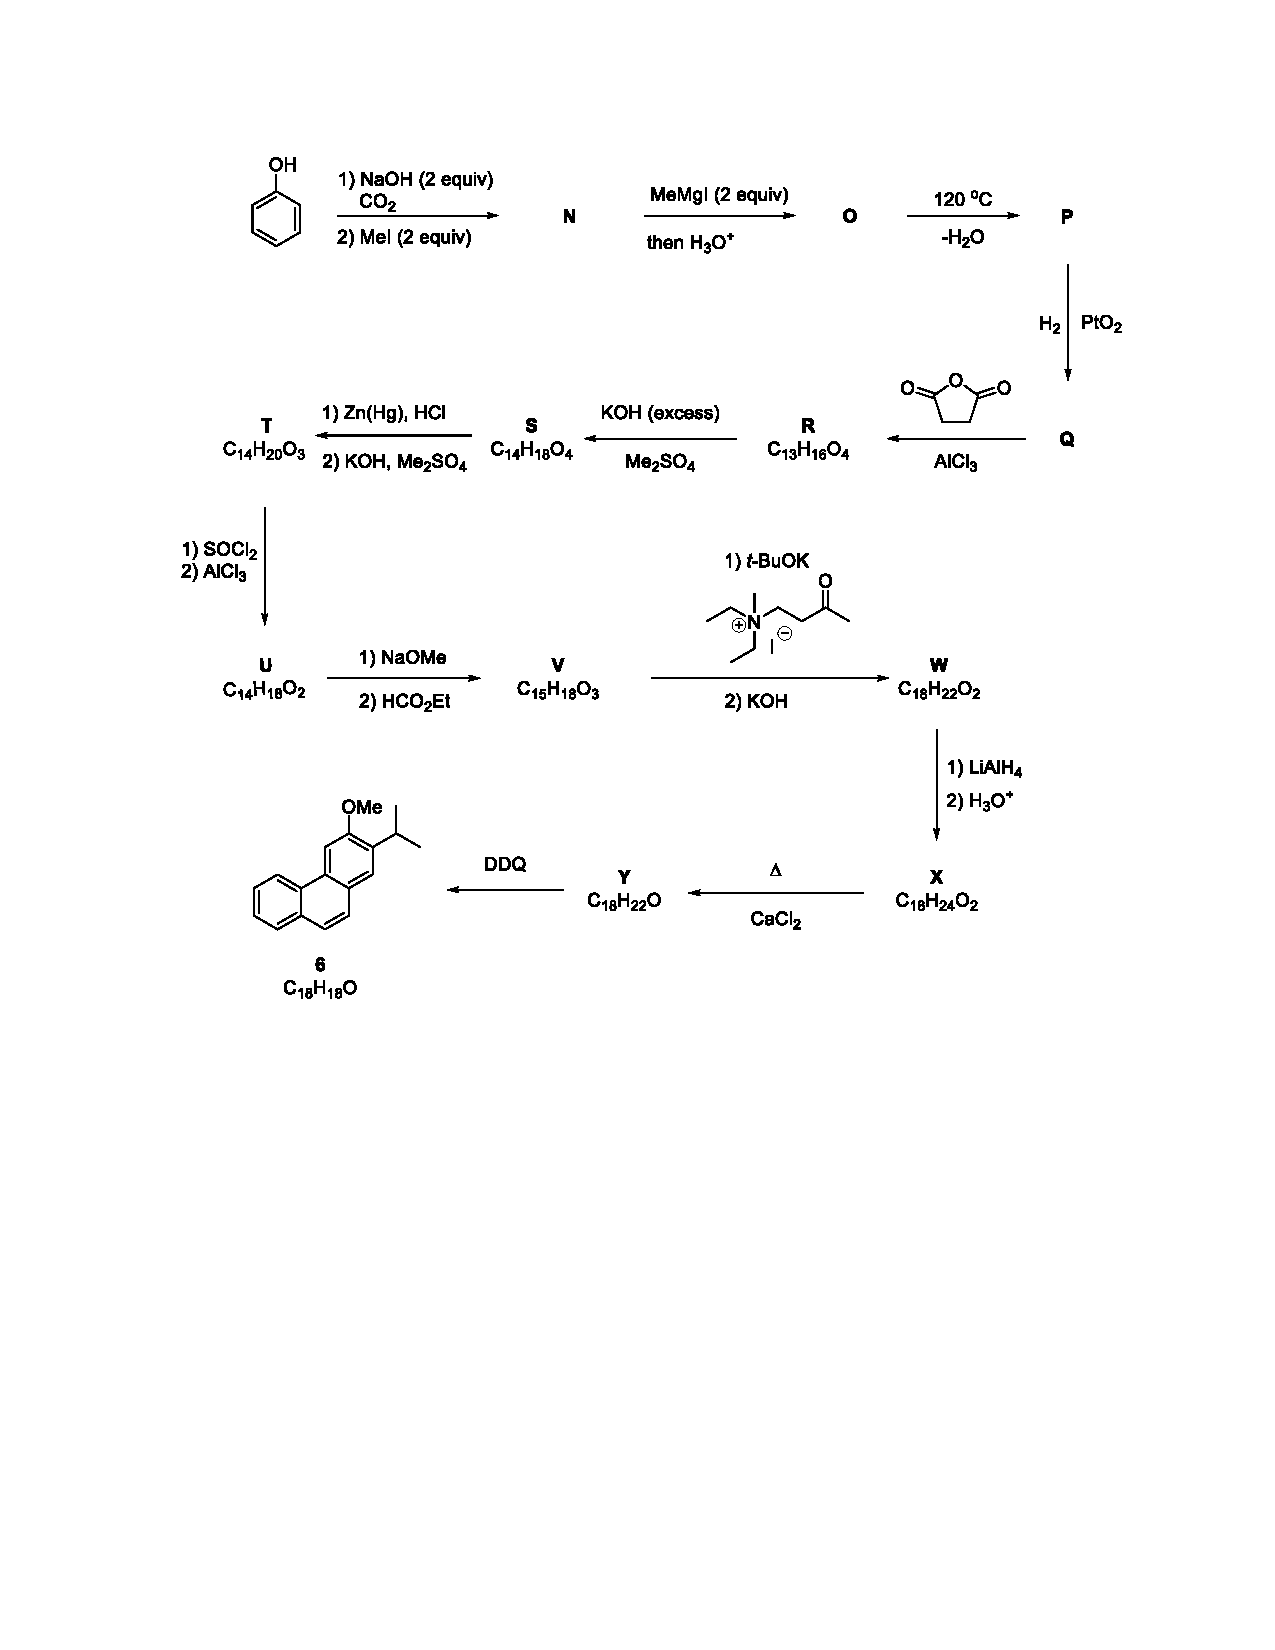
\includegraphics[width=15cm]{./pic/t1-4.pdf}
\end{figure}

\noindent\textbf{1.3.} 接下来的反应图与二萜\textbf{1}和\textbf{2}的去甲基衍生物\textbf{6}有关。画出产物\textbf{N}--\textbf{Y},无需考虑立体构型。\textbf{提示}:化合物\textbf{R}、\textbf{S}、\textbf{T}有酸性。化合物\textbf{V}到\textbf{W}的转化包含Robinson增环和一个可能的去甲酰化过程。

\newpage\noindent\textbf{1.4.} 化合物\textbf{V}到\textbf{W}的转化过程中,使用$\alpha$,$\beta$--不饱和酮的前体(例如$\beta$--氯代酮或\emph{N},\emph{N},\emph{N}--三烷基--3--氧代丁基卤化铵)更好。解释原因。

\noindent\textbf{1.5.} 画出化合物\textbf{V}可能的异构体。

\noindent\textbf{1.6.} 化合物\textbf{Y}也可由化合物\textbf{Z}经电环化关环得到。画出\textbf{Z}的结构。

\noindent\textbf{1.7.} 从\textbf{X}到\textbf{Y}的转化也可使用下列哪组试剂?(忽略S\textsubscript{N}2$'$反应)。

\renewcommand{\labelitemi}{$\square$}
\begin{itemize}
	\item i) PBr\textsubscript{3}/吡啶; ii)  \textit{n}--Bu\textsubscript{3}SnH/AIBN
	\item i) PBr\textsubscript{3}/吡啶; ii) Na/\emph{t}--BuOH
	\item i) MnO\textsubscript{2}; ii) DDQ
	\item i) TsCl/吡啶; ii) LiAlH\textsubscript{4}
	\item TsCl/吡啶; ii) DBU
\end{itemize}
\renewcommand{\labelitemi}{$\bullet$}

\begin{figure}[h]
	\centering
	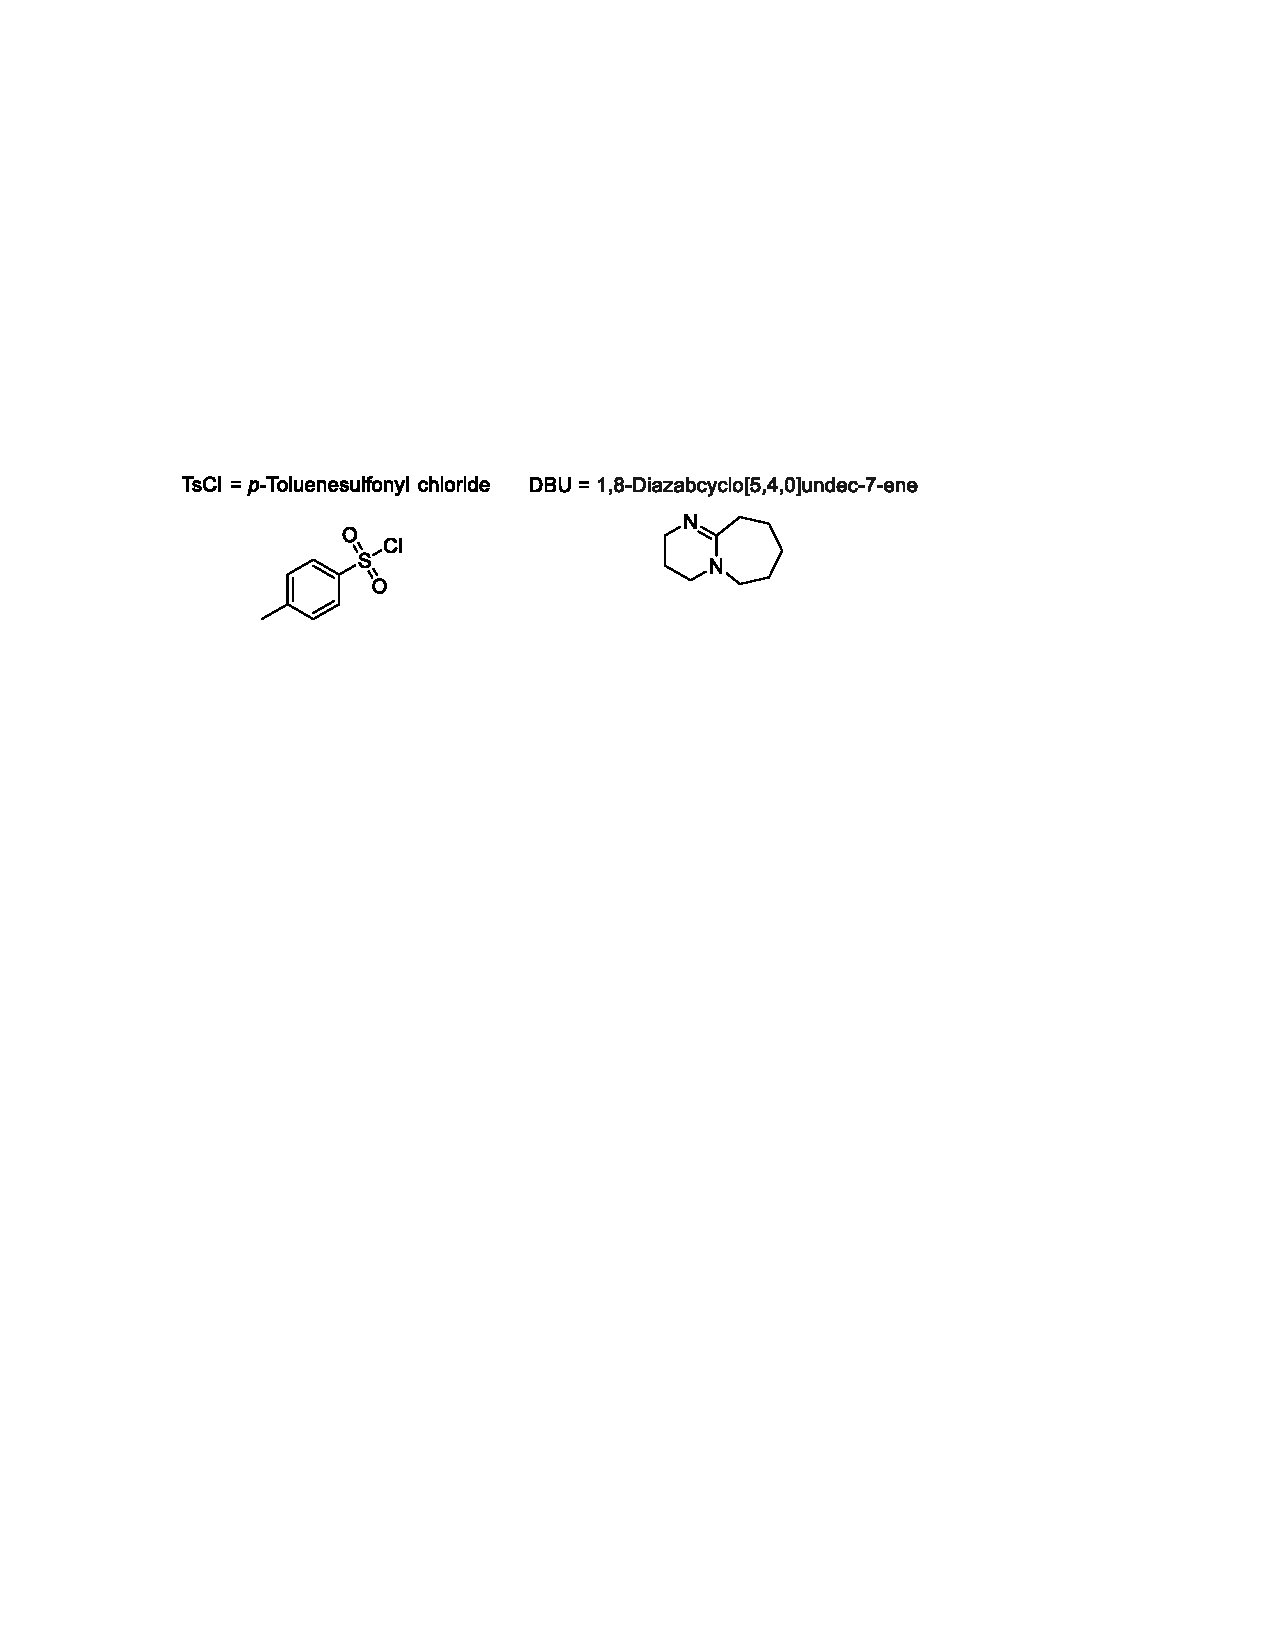
\includegraphics[width=12cm]{./pic/t1-5.pdf}
\end{figure}

